\subsection{Einleitung}
\gls{DirectShow} (ehemals \"Direct Media\")\footnote{Quelle: Wikipedia\cite{400}}
DirectShow oder ehemals ActiveMovie bzw. DirectX Media dient der Verarbeitung von Video- und Audio-Dateien, womit sich verschiedenste Arten von Video-Dateien (AVI, MPEG) und Ton-Dateien (z. B. MP3) wiedergeben oder erstellen lassen. Es wird auch Streaming unterst�tzt und ist durch DirectShow-Filter beliebig erweiterbar.
DirectShow wurde inzwischen aus dem DirectX SDK entfernt und ist in das Windows Plattform-SDK aufgenommen worden. Somit geh�rt DirectShow streng genommen nicht mehr zu DirectX, sondern ist jetzt ein Bestandteil der Windows-Plattform.

Lazarus und Freepascal unterst�tzen eine vielzahl von Umgebungen, DirectShow ist eine FrameWork nur f�r Windows 32 und 64. Somit k�nnen die folgenden Informationen nur f�r Windowsversionen gelten auf denen zumindest DirectX9 oder neuer installiert ist. 

Die meisten modernen Ger�te haben bereits eine Kamera eingebaut. Diese ist intern meistens als USB-Device angeschlossen. Wie sie genau angeschlossen ist, ist f�r den Programmiere nicht relevant, solange die Kamera vom System erkannt wird und die entsprechenden Treiber von Windows geladen werden. Entweder sind die Treiber bereits generisch in Windows enthalten oder werden vom Hersteller zur Verf�gung gestellt.   

In den Beispielen wird es spezielle um Informationen gehen die sich in erster Linie mit Kameras und den verbunden Einstellungen besch�ftigt.

\subsection{Abfragen der Kategorien}
Die verschiedenen Filter sind in Kategorien eingeteilt, diese Ergeben sich aus dem Zweck der Filter und sind vom System her vorgegeben. Kategorien werden am einfachsten �ber \textbf{TSysDevEnum} aus dem Paket \textbf{DXSUtils} abgefragt. Wir lassen uns hier den lesbaren Namen \gls{FriendlyName} statt der \gls{GUID} anzeigen. Sp�ter k�nnen wir die weiteren Informationen die wir �ber \textbf{TSysDevEnum} abfragen, durch die Angabe einer \gls{GUID} auf die ben�tigten einschr�nken. 

\lstset{language=Pascal}
\lstinputlisting{../../Demos/Lazarus/10Basics/01EnumerationCategories/basicenumcatmain.pas}
Das Ergebnis sieht wie auf der Abbildung~\ref{fig:basicenumcat01}~\nameref{fig:basicenumcat01} auf Seite~\pageref{fig:basicenumcat01} aus.
\begin{figure}[h!]
	\centering
	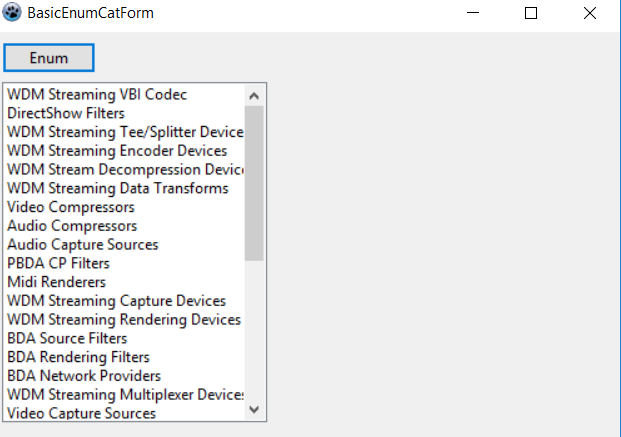
\includegraphics[width=0.7\linewidth]{../../Demos/Lazarus/01Pic/BasicEnumCat01}
	\caption[Bsp. Basic Enum Cat]{Bsp. Basic Enum Cat}
	\label{fig:basicenumcat01}
\end{figure}
Die angezeigten Kategorien sind vom System vorgegeben, daher k"onnen diese von PC zu PC abweichend sein.  

\subsection{Abfrage der Filter in der Kategorie}
Hier wird wie im vorigen Beispiel durch die verschiedenen Kategorien iteriert und das ganze in der TreeView sichtbar gemacht, zus"atzlich werden f�r jede der Kategorien die entsprechenden Filter abgefragt und in der TreeView innerhalb der entsprechen Kategorie angezeigt.

\lstset{language=Pascal}
\lstinputlisting{../../Demos/Lazarus/10Basics/02SelectCategories/basiccatmain.pas}
Das Ergebnis sieht wie auf der Abbildung~\ref{fig:basicatform01}~\nameref{fig:basicatform01} auf Seite~\pageref{fig:basicatform01} aus.
\begin{figure}[h!]
	\centering
	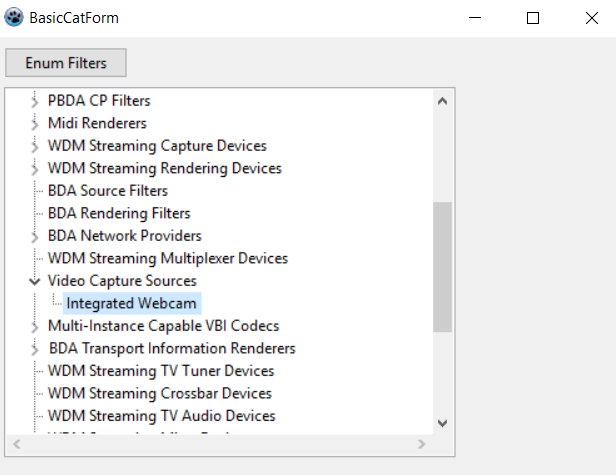
\includegraphics[width=0.7\linewidth]{../../Demos/Lazarus/01Pic/BasiCatForm01}
	\caption[Bsp. Filter in den Kategorien]{}
	\caption{}
	\label{fig:basicatform01}
\end{figure}
Die angezeigten Kategorien sind vom System vorgegeben, daher k"onnen diese von PC zu PC abweichend sein.  

\subsection{Anzeige �ber VideoInputDeviceCategory}
Hier wird eine Kategorie �ber ihre \gls{GUID} schon beim erstellen ausgew�hlt und das ganze in der TreeView sichtbar gemacht, zus"atzlich werden f�r jede der Devices die entsprechenden GUIDs abgefragt und zusammen mit dem Namen beim Klicken angezeigt.

\lstset{language=Pascal}
\lstinputlisting{../../Demos/Lazarus/10Basics/03SelectWebCam/basicselwebcammain.pas}
%%Das Ergebnis sieht wie auf der Abbildung~\ref{fig:basicatform01}~\nameref{fig:basicatform01} auf Seite~\pageref{fig:basicatform01} aus.
%%\begin{figure}[h!]
%%	\centering
%%	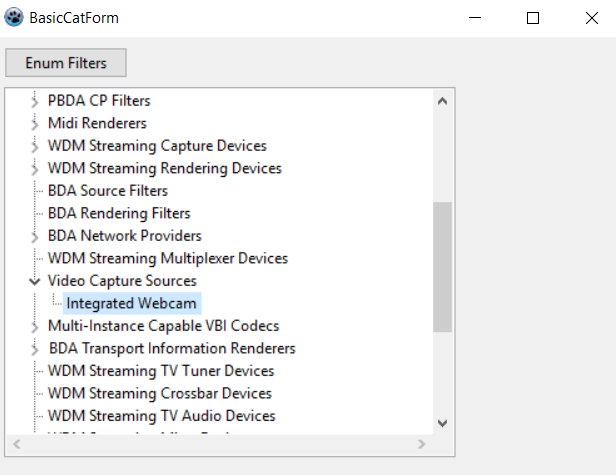
\includegraphics[width=0.7\linewidth]{../../Demos/Lazarus/01Pic/BasiCatForm01}
%%	\caption[Bsp. Filter in den Kategorien]{}
%%	\caption{}
%%	\label{fig:basicatform01}
%%\end{figure}
%%Die angezeigten Kategorien sind vom System vorgegeben, daher k"onnen diese von PC zu PC abweichend sein.  





